\documentclass[professionalfonts,compress,unicode]{beamer}
% vim: sts=4 ts=4 sw=4 et tw=80
\usepackage{amsmath,amssymb}
\usepackage[utf8]{inputenc}

\usepackage[russian]{babel}

\usepackage{multirow}
\usepackage{colortbl}
\usepackage{cancel}
\usepackage{epstopdf}

\usetheme{Warsaw}
\usecolortheme{uranix}

\setbeamertemplate{headline}
{%
  \begin{beamercolorbox}[sep=0.3cm,wd=\paperwidth]{section in head/foot}%
    \usebeamerfont{frametitle}%
    \vbox{}\vskip-1ex%
    \strut\insertsectionhead\strut\par%
    \vskip-1ex%
  \end{beamercolorbox}%
}
\setbeamertemplate{navigation symbols}{}
\setbeamertemplate{footline}{}

\renewcommand{\thefootnote}{\fnsymbol{footnote}}
\renewcommand{\arraystretch}{1.3}

\graphicspath{{images/}{source/}}

\title[СЛАУ]{Системы линейных алгебраических уравнений.\\ 
			Часть 3. Итерационные методы решения}
\author[Цыбулин И.В.]{Скалько Юрий Иванович\\
\textbf{Цыбулин Иван}}
\date{}
%\vspace{0.3cm}

\begin{document}

{
\setbeamertemplate{headline}[default]
\frame{
\titlepage
}

%\frame{
%\frametitle{Содержание}
%\small
%%\tiny
%\tableofcontents
%}
}

\newcommand\myframe[2]{\subsection{#1}\frame{\frametitle{#1}{#2}}}

\section{ }

%\myframe{Материалы по курсу вычислительной математики}
%{
%\begin{itemize}
	%\item 
		%Материалы курса (методички, лекции, учебники и др.) можно найти 
		%на сайте кафедры вычислительной математики
		%{\color{blue} http://crec.mipt.ru/study/materials/compmath/}
	%\item 
		%Любые вопросы по курсу (и не только) можно присылать на почтовый ящик
		%{\color{blue} tsybulinhome@gmail.com}
%\end{itemize}
%}

\def\A{{\bf A}}
\def\B{{\bf B}}
\def\C{{\bf C}}
\def\D{{\bf D}}
\def\E{{\bf E}}
\def\L{{\bf L}}
\def\U{{\bf U}}
\def\W{{\bf W}}
\def\S{{\bf S}}
\def\J{{\bf J}}
\def\x{{\bf x}}
\def\y{{\bf y}}
\def\v{{\bf v}}
\def\w{{\bf w}}
\def\f{{\bf f}}
\def\b{{\bf b}}
\def\r{{\bf r}}
\def\p{{\bf p}}
\def\z{{\bf z}}

\section{Методы Якоби и Зейделя}
\myframe{Задача}
{
	Рассмотрим систему уравнений $\A\x = \b$, где 
	\begin{equation*}
	\A = \begin{pmatrix}
	20 & 0 & -6\\
	0 & 20 & 7 \\
	-6 & 7 & 8 
	\end{pmatrix}
	\quad \b = \begin{pmatrix}
	26 \\ -7 \\ -14
	\end{pmatrix}
	\end{equation*}

	Выпишем для нее методы Якоби и Зейделя и исследуем их на сходимость
}

\myframe{Метод Якоби}
{
	Метод Якоби получается, если в системе уравнений $\A\x = \b$ 
	диагональные неизвестные брать с итерации $k+1$, а внедиагональные --- с $k$.
	\begin{equation*}
	\begin{cases}
	20x_1^{(k+1)} + 0x_2^{(k)}  -6 x_3^{(k)} &= 26\\
	0x_1^{(k)} + 20x_2^{(k+1)} + 7x_3^{(k)}  &= -7\\
	-6x_1^{(k)} + 7x_2^{(k)} + 8x_3^{(k+1)} &= -14 
	\end{cases}
	\end{equation*}

	Перепишем в виде метода простой итерации $\x_{k+1} = \B \x_k + \f$:

	\begin{equation*}
	\begin{cases}
	x_1^{(k+1)} &= \frac{3}{10} x_3^{(k)} + \frac{13}{10}\\
	x_2^{(k+1)} &= -\frac{7}{20} x_3^{(k)} - \frac{7}{20}\\
	x_3^{(k+1)} &= \frac{3}{4} x_1^{(k)} -\frac{7}{8} x_2^{(k)} -\frac{7}{4}
	\end{cases}
	\end{equation*}
}

\myframe{Сходимость метода Якоби}
{
	Диагонального преобладания (достаточное условие) у $\A$ нет, поэтому метод
	Якоби может не сходится. Будем проверять необходимое и достаточное условие 
	метода простых итераций $|\lambda(\B)| < 1$.

	\begin{equation*}
	\B = \begin{pmatrix}
		0 & 0 & \frac{3}{10}\\
		0 & 0 & -\frac{7}{20}\\
		\frac{3}{4} & -\frac{7}{8} & 0
	\end{pmatrix}
	\end{equation*}

	\begin{align*}
	\operatorname{det}(\B - \lambda \E) &= -\lambda\left(\lambda^2 - \frac{49}{160}\right) + \frac{9}{40}\lambda = 
	\lambda \left(\frac{85}{160} - \lambda^2\right) = 0\\
	\lambda &= \left\{ 0, \pm \sqrt{\frac{17}{32}} \right\}, \quad |\lambda(\B)| < 1
	\end{align*}

	Метод сходится при любом начальном приближении
}

\myframe{Метод Зейделя}
{
	Метод Зейделя получается, если в системе уравнений $\A\x = \b$ 
	неизвестные на диагонали и ниже брать с итерации $k+1$, 
	а остальные --- с $k$.
	\begin{equation*}
	\begin{cases}
	20x_1^{(k+1)} + 0x_2^{(k)}  -6 x_3^{(k)} &= 26\\
	0x_1^{(k+1)} + 20x_2^{(k+1)} + 7x_3^{(k)}  &= -7\\
	-6x_1^{(k+1)} + 7x_2^{(k+1)} + 8x_3^{(k+1)} &= -14 
	\end{cases}
	\end{equation*}

	Перепишем в виде метода простой итерации $\x_{k+1} = \B \x_k + \f$:
	\begin{equation*}
	\begin{cases}
	x_1^{(k+1)} &= \frac{3}{10} x_3^{(k)} + \frac{13}{10}\\
	x_2^{(k+1)} &= -\frac{7}{20} x_3^{(k)} - \frac{7}{20}\\
	x_3^{(k+1)} &= \frac{3}{4} 
	\left(\frac{3}{10} x_3^{(k)} + \frac{13}{10}\right) 
	-\frac{7}{8} \left(-\frac{7}{20} x_3^{(k)} - \frac{7}{20}\right)-\frac{7}{4}
    = \frac{17}{32} x_3^{(k)} - \frac{15}{32}
	\end{cases}
	\end{equation*}
}

\myframe{Сходимость метода Зейделя}
{
	Хотя матрица $\A = \A^\mathsf{T} > 0$ и удовлетворяет достаточному условию 
	сходимости метода Зейделя, проверим сходимость по определению.
    \begin{equation*}
    \B = \begin{pmatrix}
    0 & 0 & \frac{3}{10} \\
    0 & 0 & \frac{-7}{20} \\
    0 & 0 & \frac{17}{32}
    \end{pmatrix}
    \end{equation*}
    Найдем $\lambda(\B)$:
    \begin{align*}
    \operatorname{det} (\A - \lambda \E) &= 
    \lambda^2 \left(\frac{17}{32} - \lambda \right) = 0\\
    \lambda &= \left\{ 0, 0, \frac{17}{32}\right\}
    \end{align*}
    Все $\lambda(\B)$ лежат в единичном круге, а значит, метод сходится.
}

\myframe{Немонотонная сходимость итерационных методов}
{
	Возможны случаи, когда итерационные методы сначала удаляются от точного решения, а затем
	начинают приближаться. Это называется немонотонной сходимостью итерационного процесса. 

	Будет сходимость метода монотонной или нет, зависит от матрицы итерационного процесса $\B$, 
	используемого начального приближения и нормы, в которой изучается сходимость.

    Введем невязку $\r_k = \x_k - \x^*$, где $\x^*$ --- точное решение. Вычитая
    из $\x_{k+1} = \B \x_k + \f$ предельное равенство $\x^* = \B \x^* + \f$,
    получаем соотношение для невязки
    \begin{equation*}
        \r_{k+1} = \B \r_k
    \end{equation*}
}

\myframe{Немонотонная сходимость итерационных методов}
{
    На каждом шаге процесса невязка умножается на матрицу $\B$.
    \begin{equation*}
        \r_{k+1} = \B \r_k
    \end{equation*}

    Нас интересует, будет ли норма невязки $\varepsilon_k = \|\r_k\|_\bullet$
    стремится к нулю монотонно или нет. Рассмотрим случаи 
    \begin{itemize}
        \item $q = \|B\|_\bullet < 1$. В этом случае сходимость монотонная:
            $$\varepsilon_{k+1} = \|\r_{k+1}\|_\bullet = 
                \|\B\r_k\|_\bullet \leq \|\B\|_\bullet \|\r_k\|_\bullet = q
                \varepsilon_k < \varepsilon_k$$
        \item $q = \|B\|_\bullet \geq 1$. Возьмем $\r_0 \neq 0$ такое, чтобы
            $$ \|\B\r_0\|_\bullet = \|\B\|_\bullet \|\r_0\|_\bullet$$
            Получаем, что $\varepsilon_1 = \|\r_1\|_\bullet = \|\B\r_0\|_\bullet
            = q\|\r_0\|_\bullet = q \varepsilon_0 \geq \varepsilon_0$
            Для начального приближения $\x_0 = \x^* + \r_0$ сходимость будет
            немонотонная.
    \end{itemize}
}

\myframe{Немонотонная сходимость}
{
    Например, для рассмотренного метода Якоби
    \begin{equation*}
	\B = \begin{pmatrix}
		0 & 0 & \frac{3}{10}\\
		0 & 0 & -\frac{7}{20}\\
		\frac{3}{4} & -\frac{7}{8} & 0
	\end{pmatrix}
    \end{equation*}
    сходимость в норме $\|\,\|_1$ будет монотонная 
    ($\|\B\|_1 = \frac{7}{8} <1$), а в норме $\|\,\|_\infty$ --- не всегда.
    Норма $\|\B\|_\infty = \frac{13}{8}$ достигается на векторе 
    $\r_0 = (1,-1,0)^\mathsf{T}$. В качестве начального приближения можно 
    взять 
    \begin{equation*}
        \x_0 = \x^* + r_0 = (1, 0, -1)^\mathsf{T} + (1,-1,0)^\mathsf{T} =
        (2,-1,-1)^\mathsf{T}
    \end{equation*}
}

\myframe{Число итераций}
{
    Предположим, что некоторая норма $\|\B\|_\bullet = q < 1$ оказалась
    меньше единицы. Как оценить число итераций $N$, необходимых, чтобы обеспечить
    $\varepsilon_N = \|\x_N - \x^*\|_\bullet < \varepsilon$, где $\varepsilon$ задано?

    Воспользуемся соотношением
    \begin{equation*}
    \r_{k+1} = \B \r_k \Rightarrow 
    \varepsilon_{k+1} \leq q \varepsilon_k \leq \dots \leq 
    q^{k+1} \|\x_0 - \x^*\|_\bullet
    \end{equation*}

    В этой оценке имеется решение $\x^*$, которое заранее не известно. Избавимся
    от него следующим способом
    \begin{align*}
    \|\x_0 - \x_*\|_\bullet \leq 
    \|\x_0 - \x_1\|_\bullet + \|\x_1 - \x_*\|_\bullet &\leq
    \|\x_1 - \x_0\|_\bullet + q\|\x_0 - \x_*\|_\bullet\\
    (1-q)\|\x_0 - \x_*\| &\leq \|\x_1 - \x_0\|
    \end{align*}

    Получаем оценку
    \begin{equation*}
    \varepsilon_N \leq \frac{q^N}{1-q} \|\x_1 - \x_0\|_\bullet, 
    \quad N = \left\lceil \frac{\ln ((1-q) \varepsilon) - 
    \ln \|\x_1 - \x_0\|_\bullet}{\ln q}\right\rceil
    \end{equation*}
}


\section{Метод простой итерации с параметром $\tau$}

\myframe{Метод простой итерации}
{
    Пусть матрица $\A = \A^\mathsf{T} > 0$. Запишем метод простой итерации с
    параметром $\tau$
	$$
	\x_{k+1} = (\E - \tau \A) \x_k + \tau \b
	$$
    Здесь $\B = \E - \tau \A$.
	У матрицы $\B$ такие же собственные вектора, что и у матрицы $\A$, а их 
	собственные числа связаны отношением
	\footnote{Если $\A \x = \lambda \x$, то
	$
	\B \x = (\E - \tau \A) \x = \x - \tau \lambda \x = (1 - \tau \lambda) \x
	$}
	$$
	\lambda(\B) = 1 - \tau \lambda(\A)
	$$
    Необходимое и достаточное условие сходимости $|\lambda(\B)| < 1$
    ограничивает
    $$
    0 < \tau < \frac{2}{\max \lambda(\A)} \equiv \frac{2}{\lambda_{max}}
    $$
}

\myframe{Скорость сходимости}
{
    Поскольку матрица $\A$ симметрична (следовательно и матрица $\B$), ее
    собственные вектора $\w_i$ образуют ортогональную систему. Обозначим
    $q_i = 1- \tau \lambda_i$.
    $$ \A \w_i = \lambda_i \w_i, \quad \B \w_i = q_i \w_i = (1 - \tau \lambda_i) \w_i$$
    Разложим вектор невязки
    по этому базису из собственных векторов матриц $\A$ и $\B$:
    \begin{align*}
    \r_k &= \sum_{i=1}^n \alpha_i^{(k)} \w_i\\
    \r_{k+1} &= \B\r_k = \sum_{i=1}^n \B \alpha_i^{(k)} \w_i = \sum_{i=1}^n
    (1-\tau\lambda_i)\alpha^{(k)}_i \w_i
    \end{align*}
    Получается, что $\alpha^{(k)}_i = q_i^k \alpha^{(0)}_i$, то есть $i$-я
    компонента невязки стремится к нулю со скоростью $|q_i|$.
}

\myframe{Метод простой итерации при $\tau \ll \frac{1}{\lambda_{max}}$}
{
\begin{columns}
\begin{column}{0.5\textwidth}
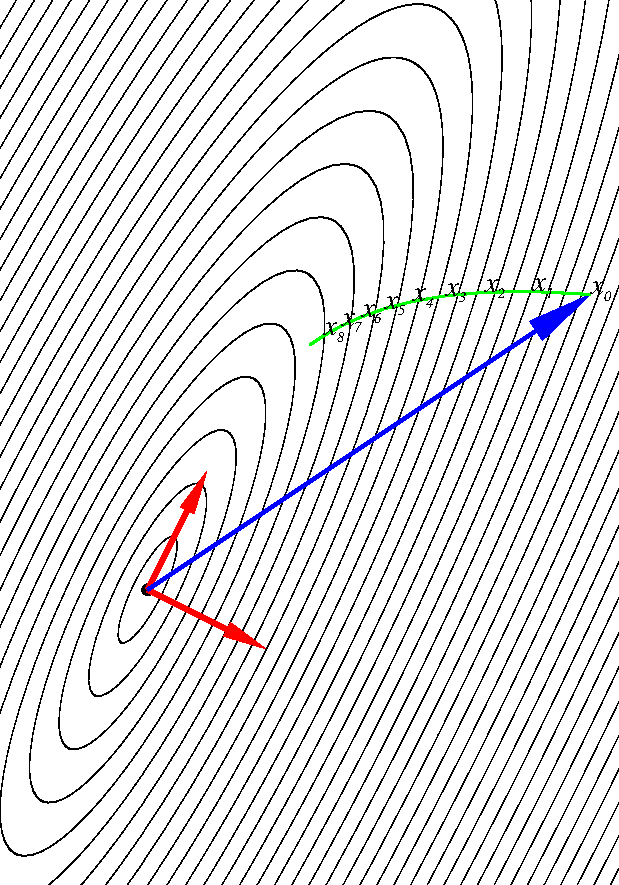
\includegraphics[width=\columnwidth]{si0_05.pdf}%
\end{column}
\begin{column}{0.5\textwidth}
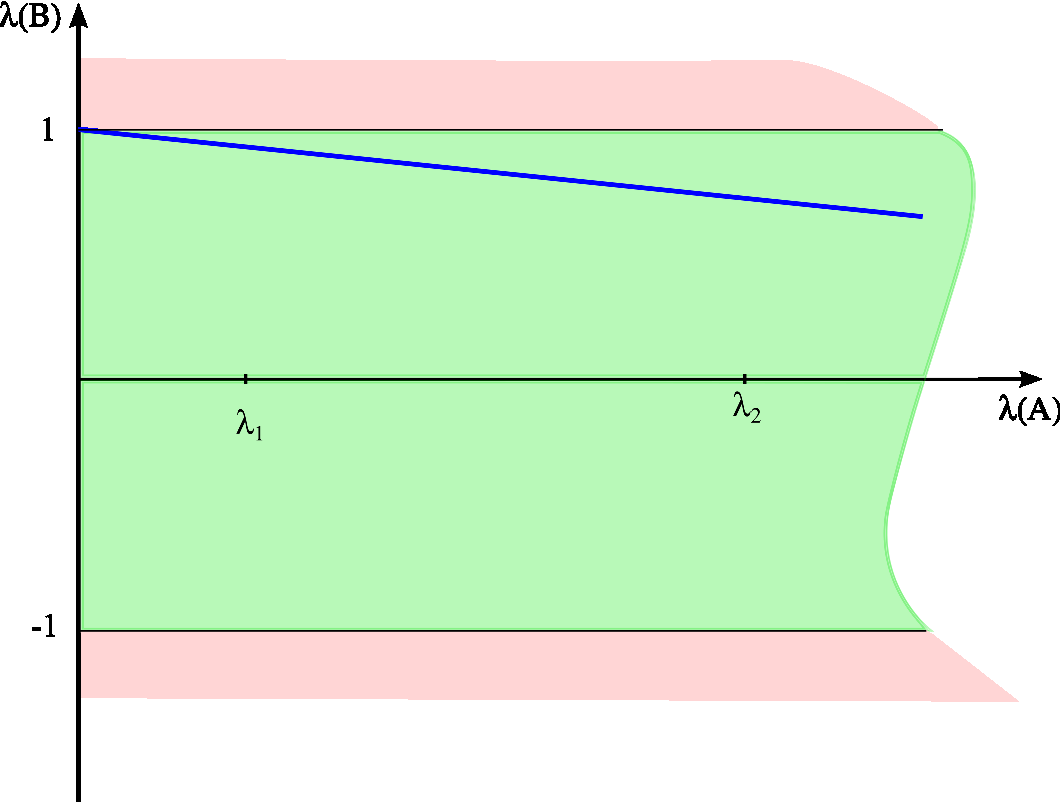
\includegraphics[width=\columnwidth]{lAlB0_05.pdf}%
\end{column}
\end{columns}
}

\myframe{Метод простой итерации при $\tau \approx \frac{1}{\lambda_{max}}$}
{
\begin{columns}
\begin{column}{0.5\textwidth}
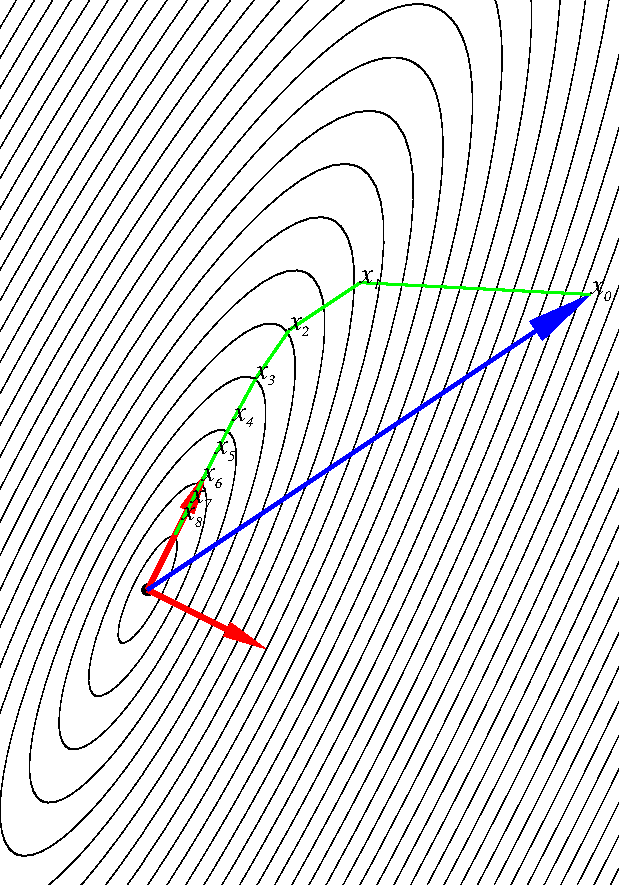
\includegraphics[width=\columnwidth]{si0_20.pdf}%
\end{column}
\begin{column}{0.5\textwidth}
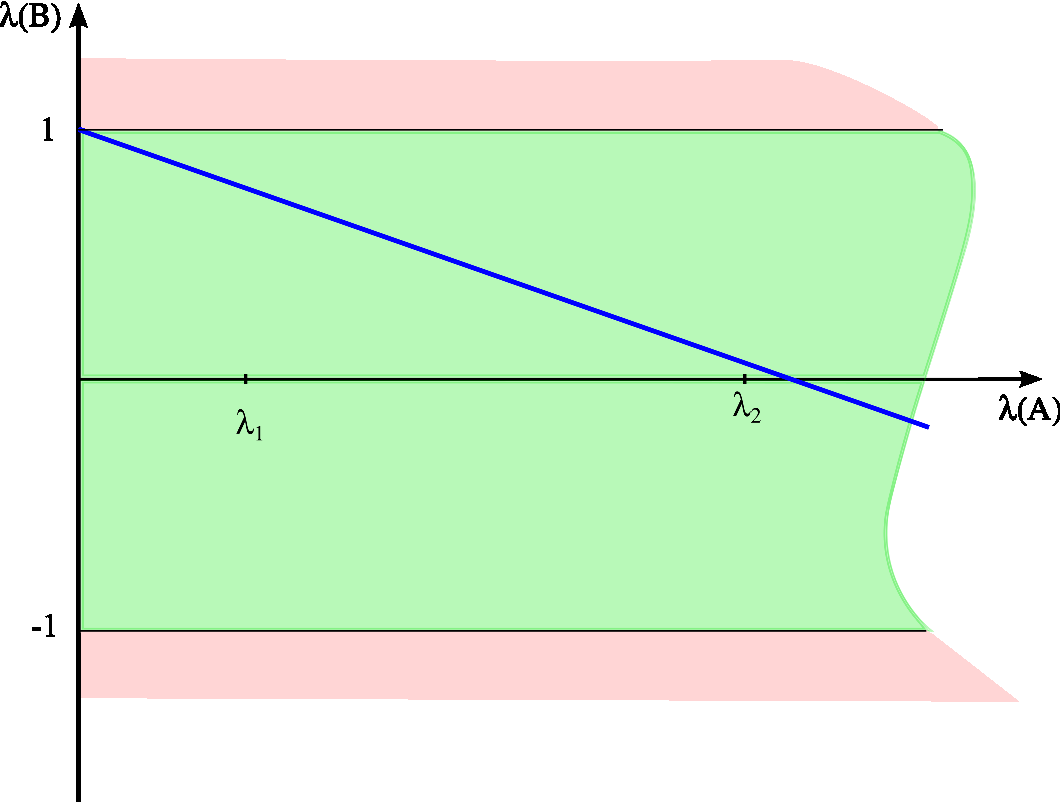
\includegraphics[width=\columnwidth]{lAlB0_20.pdf}%
\end{column}
\end{columns}
}

\myframe{Метод простой итерации при 
$\tau < \tau_{opt} = \frac{2}{\lambda_{\min} + \lambda_{\max}}$
}
{
\begin{columns}
\begin{column}{0.5\textwidth}
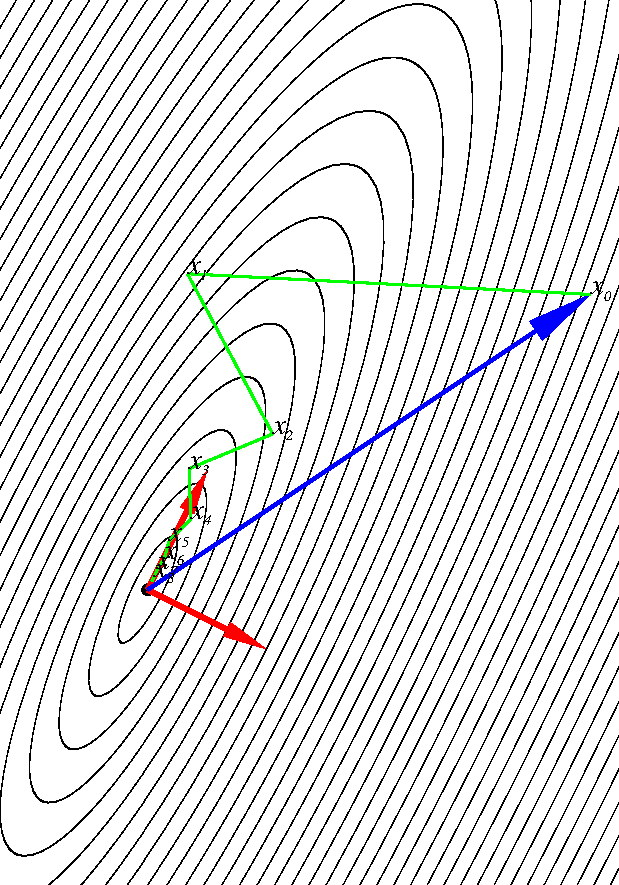
\includegraphics[width=\columnwidth]{si0_35.pdf}%
\end{column}
\begin{column}{0.5\textwidth}
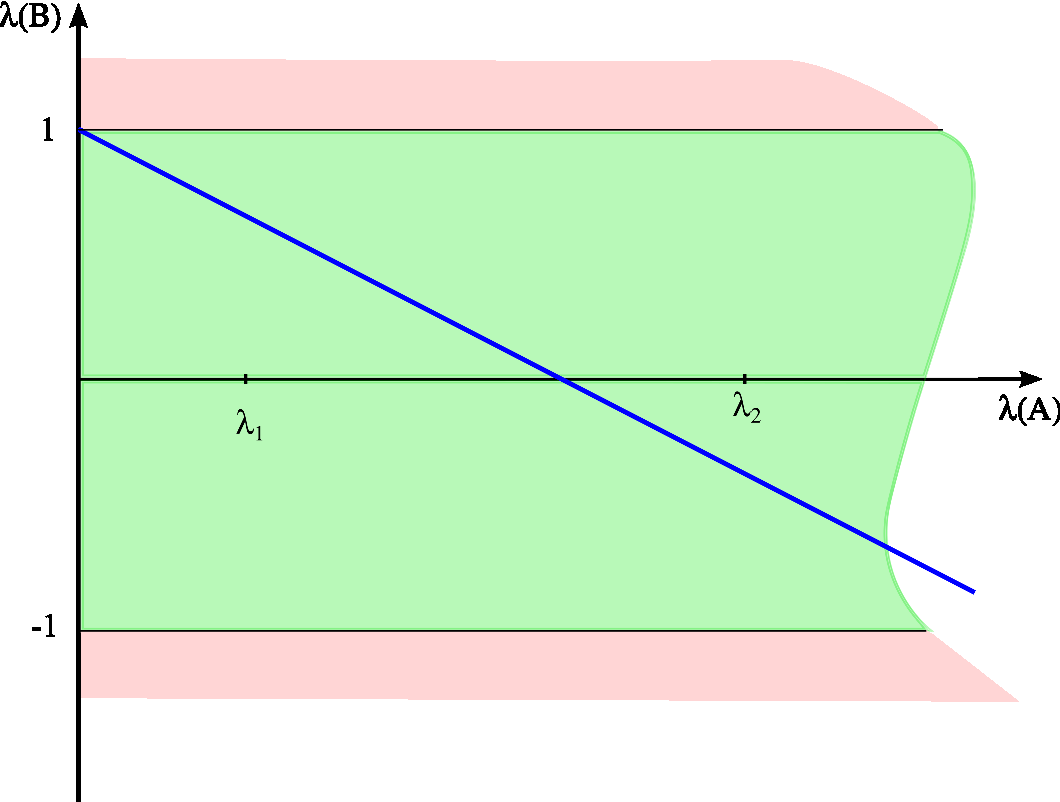
\includegraphics[width=\columnwidth]{lAlB0_35.pdf}%
\end{column}
\end{columns}
}

\myframe{Метод простой итерации при 
$\tau = \tau_{opt} = \frac{2}{\lambda_{\min} + \lambda_{\max}}$
}
{
\begin{columns}
\begin{column}{0.5\textwidth}
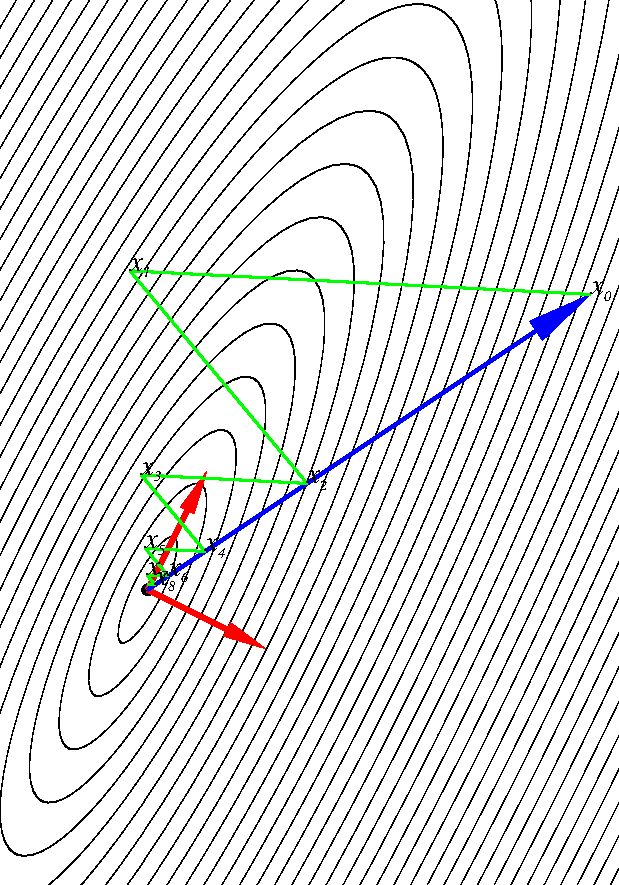
\includegraphics[width=\columnwidth]{si0_40.pdf}%
\end{column}
\begin{column}{0.5\textwidth}
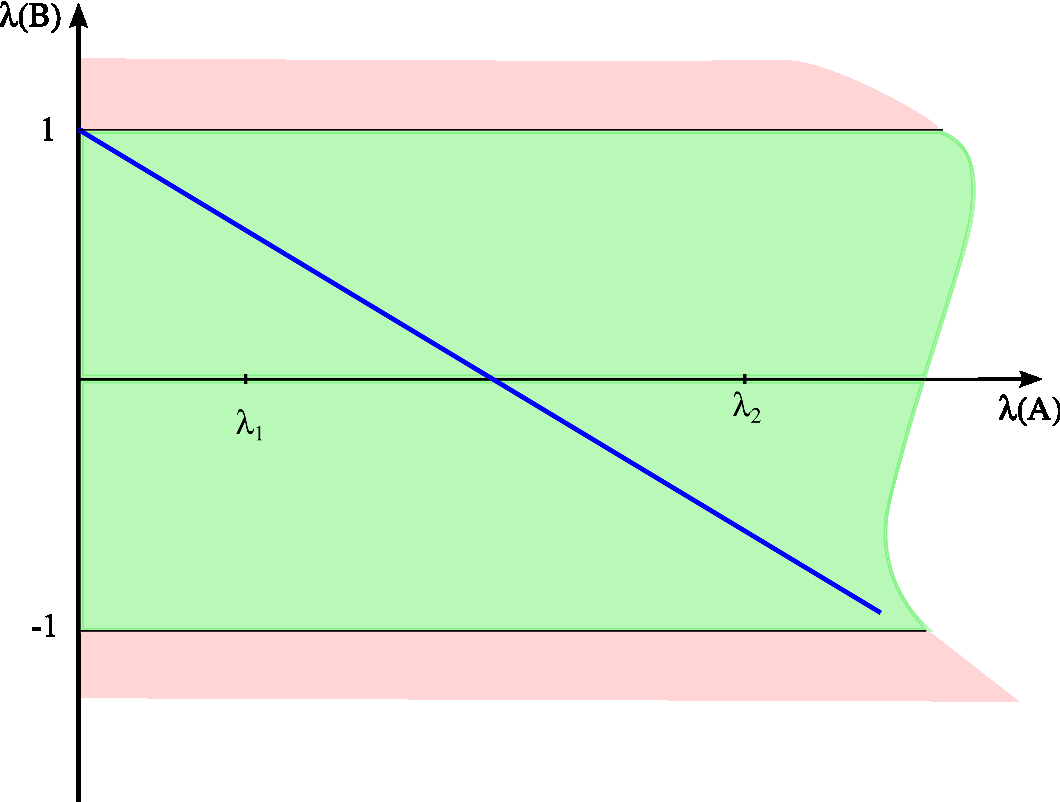
\includegraphics[width=\columnwidth]{lAlB0_40.pdf}%
\end{column}
\end{columns}
}

\myframe{Метод простой итерации при 
$\tau > \tau_{opt} = \frac{2}{\lambda_{\min} + \lambda_{\max}}$
}
{
\begin{columns}
\begin{column}{0.5\textwidth}
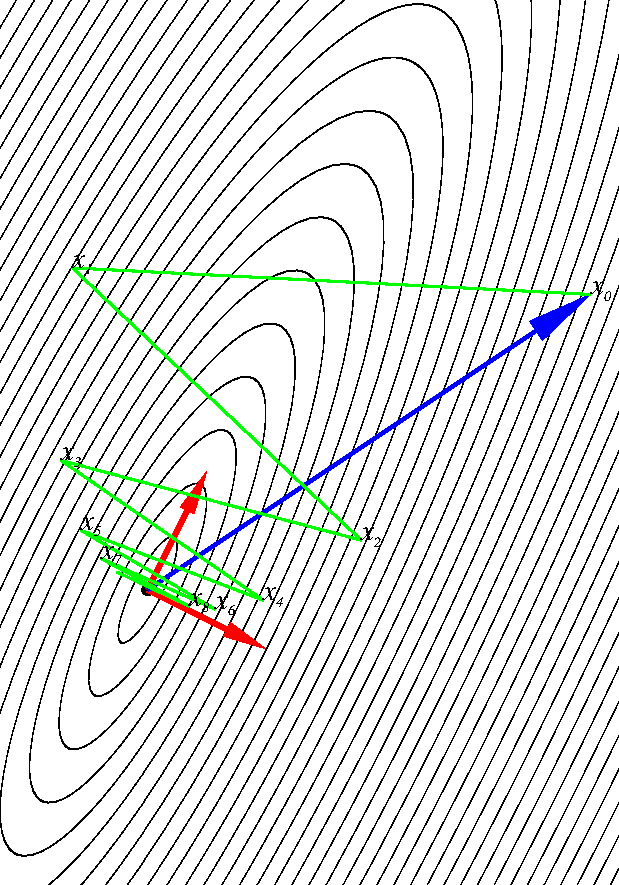
\includegraphics[width=\columnwidth]{si0_45.pdf}%
\end{column}
\begin{column}{0.5\textwidth}
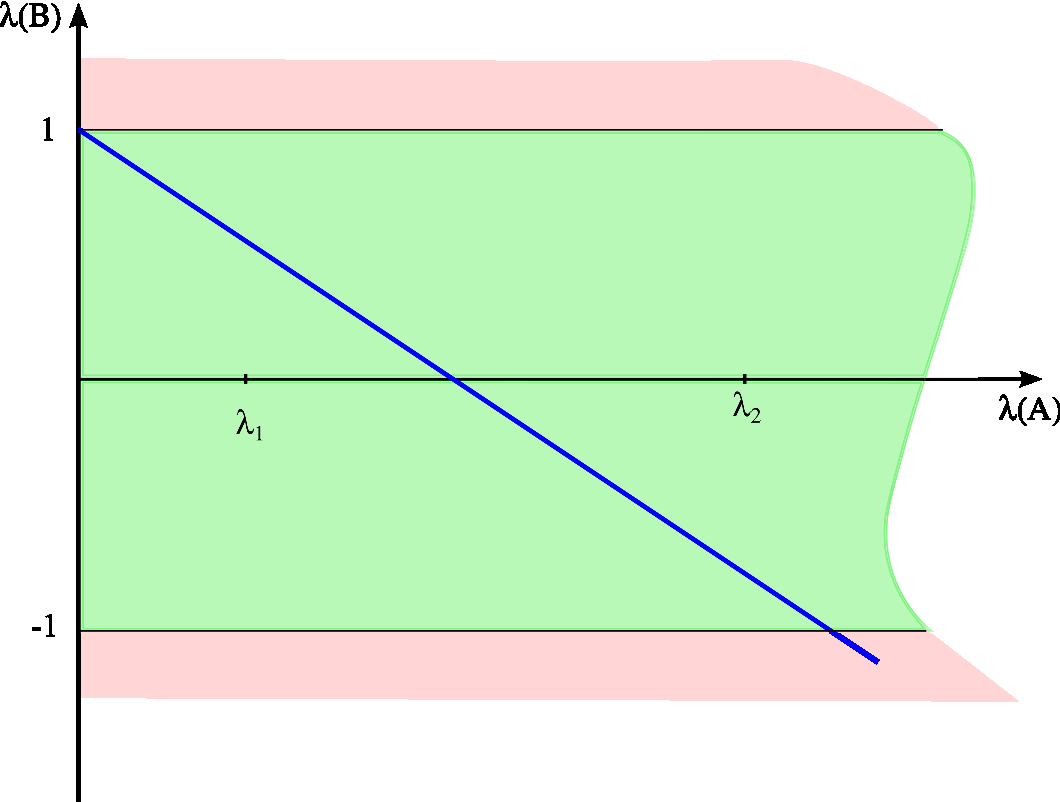
\includegraphics[width=\columnwidth]{lAlB0_45.pdf}%
\end{column}
\end{columns}
}

\myframe{Метод простой итерации при $\tau > \frac{2}{\lambda_{max}}$}
{
\begin{columns}
\begin{column}{0.5\textwidth}
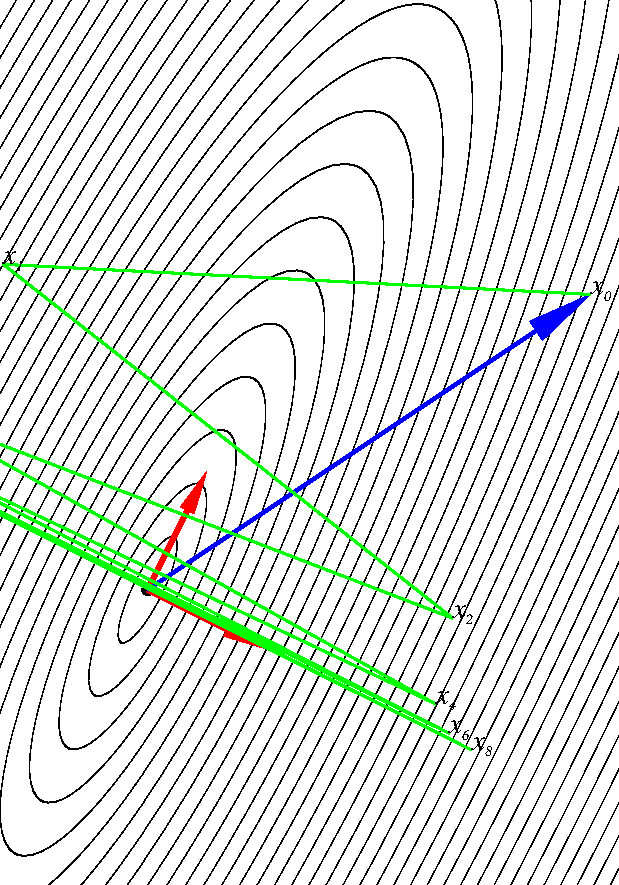
\includegraphics[width=\columnwidth]{si0_51.pdf}%
\end{column}
\begin{column}{0.5\textwidth}
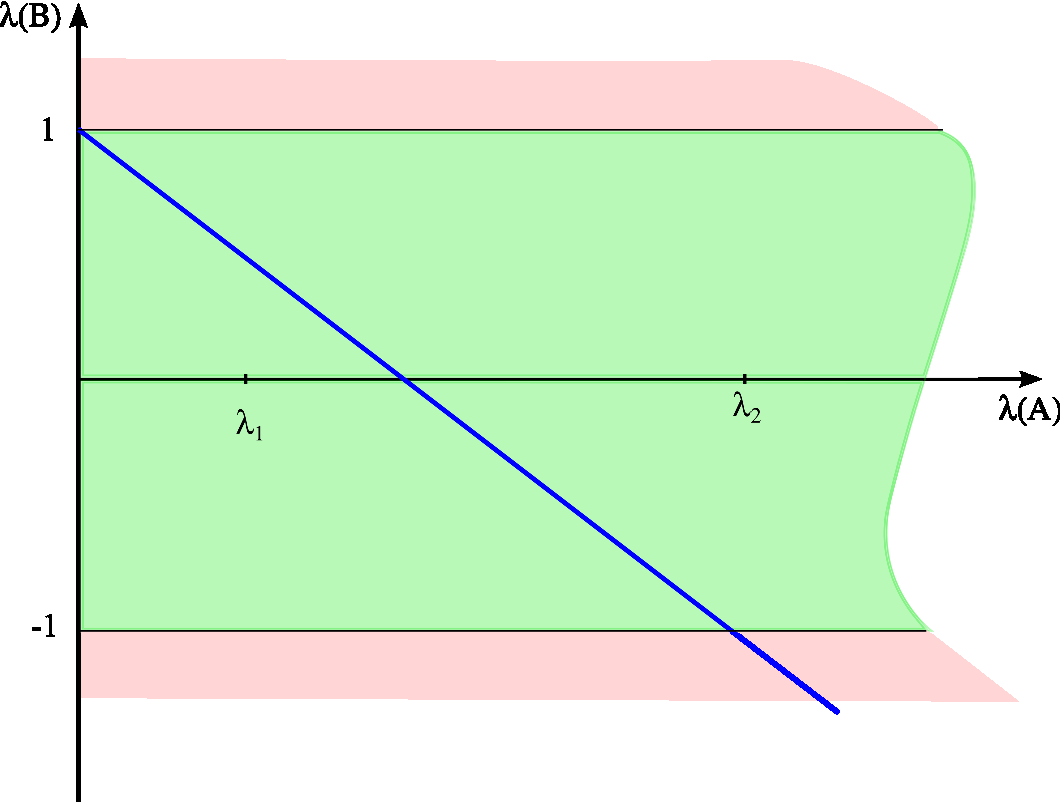
\includegraphics[width=\columnwidth]{lAlB0_51.pdf}%
\end{column}
\end{columns}
}

\myframe{Поведение при различных значениях параметра}
{
	Можно сделать несколько выводов
	\begin{itemize}
		\item При малом $\tau$ ($\tau \ll \frac{1}{\lambda_{max}}$) метод сходится очень медленно, и основным ``тормозом''
		является часть невязки, которая соответствует первому собственному вектору ($\lambda = \lambda_{min}$). Скорость сходимости
		$q = 1 - \tau \lambda_{min}$
		\item При достаточно большом $\tau$ ($\tau > \frac{2}{\lambda_{\max}}$) метод расходится
		\item При отрицательном $\tau$ ($\tau < 0$) метод расходится
		\item При большом $\tau$ ($\tau \lesssim \frac{2}{\lambda_{\max}}$) метод сходится медленно, здесь ``тормозом'' является уже
		максимальное собственное число. Скорость сходимости $q = \tau \lambda_{\max} - 1$
		\item При некотором $\tau$ ($\tau = \tau_{opt} = \frac{2}{\lambda_{\min}+\lambda_{\max}}$) 
        компоненты невязки с $\lambda = \lambda_{\min}$ и
		$\lambda = \lambda_{\max}$ стремятся к нулю с одинаковой скоростью. 
		Промежуточные компоненты стремятся к нулю еще быстрее. Этот вариант оптимален
		по скорости сходимости $q = q_{opt} = \frac{\lambda_{\max} -
        \lambda_{\min}}{\lambda_{\max} + \lambda_{\min}}$ 
	\end{itemize}
}

\myframe{Сходимость при специальных приближениях}
{  
    \begin{block}{}
    Возможно ли, что в некоторых условиях при $\tau \neq \tau_{opt}$ 
    невязка будет стремиться к нулю быстрее, чем при $\tau = \tau_{opt}$?
    \end{block}

    Оказывается, что да, но только при определенных начальных приближениях.
    Просиходит это, когда некоторые коэффициенты $\alpha^{(0)}_i$
    в разложении невязки по собственным векторам матрицы обращаются в 
    ноль. При этом не важно, чему равно соответствующее $q_i$,
    $\alpha^{(k)}_i = q_i^k \alpha^{(0)}_i$ будет продолжать оставаться нулем.

    Однако, важно не нарушать условие $|q_i| \leq 1$. В противном случае
    $\alpha^{(k)}_i$ может легко вырасти из ``машинного нуля'' до больших чисел
    и остановить сходимость процесса.
}

\myframe{Сходимость при специальных приближениях}
{
    Вернемся к системе $\A\x = \b$ с 
    \begin{equation*}
	\A = \begin{pmatrix}
	20 & 0 & -6\\
	0 & 20 & 7 \\
	-6 & 7 & 8 
	\end{pmatrix}
	\quad \b = \begin{pmatrix}
	26 \\ -7 \\ -14
	\end{pmatrix}
    \end{equation*}
    Собственные числа $\lambda_i$ и вектора $\w_i$ для этой системы:
    \begin{align*}
    &\lambda_{min} = \lambda_1 = 3 < 
    \lambda_2 = 20 < \lambda_3 = 25 =\lambda_{max}\\
    &
    \w_1 = \begin{pmatrix}
    6\\-7\\17
    \end{pmatrix} \quad
    \w_2 = \begin{pmatrix}
    7\\6\\0
    \end{pmatrix} \quad
    \w_3 = \begin{pmatrix}
    6\\-7\\-5
    \end{pmatrix}
    \end{align*}
}

\myframe{Сходимость при специальных приближениях}
{
    Рассмотрим начальное приближение $\x_0 = (0, -13, 16)^\mathsf{T}$. Соответствующая 
    невязка 
    \begin{equation*}
        \r_0 = \x_0 - \x^* = \begin{pmatrix}
            0\\ -13\\ 16
        \end{pmatrix} - 
        \begin{pmatrix}
            1\\ 0\\-1
        \end{pmatrix} =
        \begin{pmatrix}
            -1\\ -13\\ 17
        \end{pmatrix} = \w_1 - \w_2
    \end{equation*}
    В начальной невязке отсутствует компонента, соответствующая максимальному
    собственному числу ($\lambda_3$)

    Скорость сходимости $q$ определяется самой медленно сходящейся компонентой
    из оставшихся
    \begin{equation*}
        q = \max(|q_1|, |q_2|, \cancel{|q_3|}) = 
        \max(|1 - \tau \lambda_1|, |1 - \tau \lambda_2|)
    \end{equation*}
}

\myframe{Сходимость при $\alpha_3 = 0$}
{
    Найдем, при каких $\tau$ величина 
    $q = \max(|1 - \tau \lambda_1|, |1 - \tau \lambda_2|)$ 
    оказывается меньше $q_{opt}$ (то есть сходимость быстрее).
    \begin{center}
    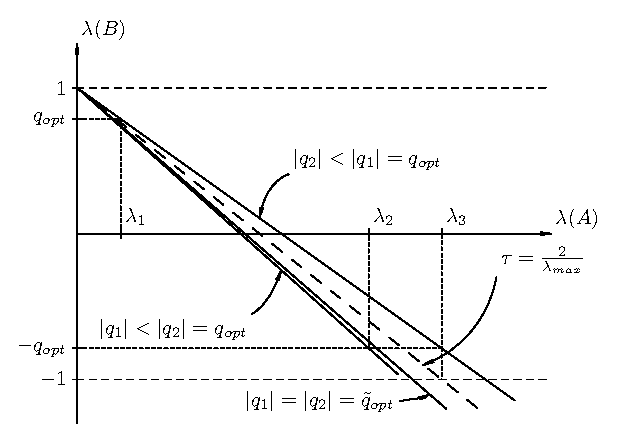
\includegraphics[height=2.5in]{special-0.eps}
    \end{center}
}

\myframe{Сходимость при $\alpha_3 = 0$}
{
    Величина $q = \max(|q_1,q_2|)$ оказывается меньше $q_{opt}$
    в диапазоне 
    \begin{equation*}
        \tau \in \left(\tau_{opt}, \frac{1+q_{opt}}{\lambda_2}\right)
    \end{equation*}

    Сходимость при этих $\tau$ и данном начальном приближении будет
    действительно быстрее, чем при $\tau_{opt}$.

    Однако, при $\tau > \frac{2}{\lambda_3}$ итерационный процесс потеряет
    устойчивость ($q_3$ станет больше $1$), третья компонента в невязке
    (которая имелась из-за численных ошибок), 
    быстро вырастет при $q_3 > 1$. Поэтому для вычислительно устойчивого 
    процесса 
    \begin{equation*}
        \tau \in \left(\tau_{opt}, \frac{1+q_{opt}}{\lambda_2}\right) \cap
        \left[0, \frac{2}{\lambda_3}\right]
    \end{equation*}
}

\myframe{Сходимость при $\alpha_3 = 0$}
{
    Найдем численное выражение для границ $\tau$ для конкретной матрицы из
    задачи:
    \begin{align*}
        \tau_{opt} &= \frac{2}{\lambda_1 + \lambda_3} = \frac{2}{3+25} =
            \frac{1}{14} \approx 0.0714\\
        q_{opt} &= \frac{\lambda_3 - \lambda_1}{\lambda_1 + \lambda_3} =
            \frac{25-3}{25+3} = \frac{11}{14} \approx 0.7857\\
        \tau &\in 
            \left(\tau_{opt}, \frac{1+q_{opt}}{\lambda_2}\right) \cap
            \left[0, \frac{2}{\lambda_3}\right] =
            \left(\frac{1}{14}, \frac{5}{56}\right) \cap
            \left[0, \frac{2}{25}\right] =
            \left(\frac{1}{14}, \frac{2}{25}\right]
    \end{align*}
    Быстрее всего метод при таком начальном приближении 
    сходится при $q_1 = -q_2$ и 
    $\tilde{\tau}_{opt} = \frac{2}{\lambda_1 + \lambda_2} = \frac{2}{23}$. 
    Поскольку это значение больше $\frac{2}{\lambda_3}$, 
    \emph{вычислительно устойчивый} метод
    быстрее всего сходится при $\tau = \frac{2}{\lambda_3}$. Это
    ближайшее значение из множества устойчивых параметров
    $\left[0,\frac{2}{\lambda_3}\right]$ к 
    $\tilde{\tau}_{opt}$.
}

\myframe{Сходимость при специальных приближениях}
{
    Рассмотрим теперь другое начальное приближение 
    $\x_0 = (14, -1, -6)^\mathsf{T}$. Начальная невязка
    \begin{equation*}
        \r_0 = \x_0 - \x^* = 
        \begin{pmatrix}
            14 \\ -1 \\ -6
        \end{pmatrix} -
        \begin{pmatrix}
            1 \\ 0 \\ -1
        \end{pmatrix} =
        \begin{pmatrix}
            13 \\ -1 \\ -5
        \end{pmatrix} = 
        \w_2 + \w_3
    \end{equation*}
    Теперь в невязке отсутствует первая компонента ($\lambda_3$). По аналогии 
    с предыдущим пунктом,
    \begin{equation*}
        q = \max(\cancel{|q_1|}, |q_2|, |q_3|) = 
            \max(|1-\tau \lambda_2|, |1 -\tau \lambda_3|)
    \end{equation*}
}

\myframe{Сходимость при $\alpha_1 = 0$}
{
    Найдем, при каких $\tau$ величина 
    $q = \max(|1 - \tau \lambda_2|, |1 - \tau \lambda_3|)$ 
    оказывается меньше $q_{opt}$ (то есть сходимость быстрее).
    \begin{center}
    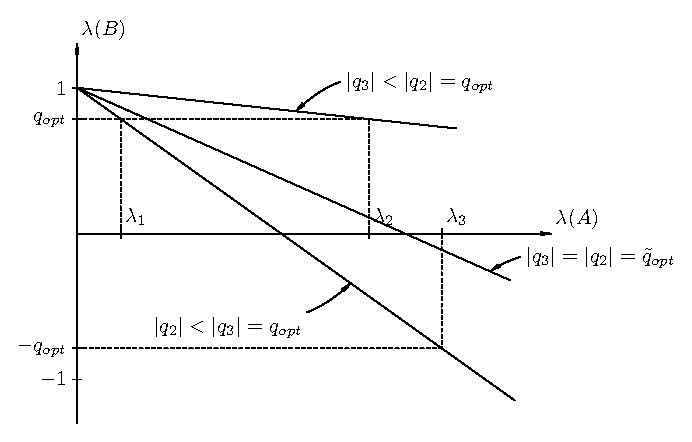
\includegraphics[height=2.5in]{special-1.eps}
    \end{center}
}

\myframe{Сходимость при $\alpha_1 = 0$}
{
    В диапазоне 
    \begin{equation*}
        \tau \in \left(\frac{1-q_{opt}}{\lambda_2},\tau_{opt}\right)
    \end{equation*}
    величина $q$ оказывается меньше $q_{opt}$, то есть сходимость быстрее.
    Отметим, что данный диапазон оказыается лежащим целиком в 
    отрезке устойчивых методов $\left[0, \frac{2}{\lambda_3}\right]$.
    
    При данном начальном приближении максимальная скорость сходимости 
    достигается при $q_2 = -q_3$ и $\tilde{\tau}_{opt} = 
    \frac{2}{\lambda_2 + \lambda_3}$. Это значение $\tilde\tau_{opt}$
    всегда приводит к устойчивому методу.

    Для данной задачи
    \begin{equation*}
        \tau \in \left(\frac{3}{280},\frac{1}{14}\right), \quad
        \tilde{\tau}_{opt} = \frac{2}{45}
    \end{equation*}
    
}
%%%%%%%%%%%%%%%%%%%%%%%%%%%%%%%%%%%%%%%%%%%%%%%
%%%%%%%%%%%%%%%%%%%%%%%%%%%%%%%%%%%%%%%%%%%%%%%
%%%%%%%%%                            %%%%%%%%%%
%%%%%%%%%%%%%%%%%%%%%%%%%%%%%%%%%%%%%%%%%%%%%%%
%%%%%%%%%%%%%%%%%%%%%%%%%%%%%%%%%%%%%%%%%%%%%%%
{
\setbeamertemplate{headline}[default] 
\frame{
	\begin{center}
	{\Huge Спасибо за внимание!}
	\end{center}
	\bigskip
	\begin{center}
	{\color{blue}{tsybulin@crec.mipt.ru}}
	\end{center}
	}
}

\end{document}
